



\section*{Problem Defintion}
\subsection*{Domain}
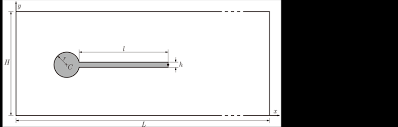
\includegraphics[scale=0.9]{geometry.png}
The computational domain resembles the classic cfd benchmark with an added bar, with dimensions: \\
The box: L = 2.5, H = 0.41 \\
The bar: l = 0.35, h = 0.02 \\
The circle is positioned at (0.2, 0.2) making it 0.05 of center from bottom to top, this is done to induce oscillations to an otherwise laminar flow.\\
Boundary conditions:\\
The fluid velocity has a parabolic profile on the inlet that changes over time:\\
$$ u(0,y) = 1.5u_0 \frac{y(H-y)}{(\frac{H}{2})^2}  $$
$$ u(0,y,t) = u(0,y)\frac{1-cos(\frac{\pi}{2}t)}{2} \text{  for  } t<2.0$$
$$ u(0,y,t) = u(0,y) \text{  for  } t \leq 2.0 $$

We set no slip on the "floor" and "ceiling" so to speak.\\
On the fluid solid interface the boundary conditions are set to:
$$  \sigma_f n_f = \sigma_s n_s \hspace{4mm} on  \hspace{2mm}\Gamma^0 (interface)   $$
In our variational form we leave this out and so implying that they are equal.

\subsection*{CSM test}
Parameters
\begin{table}[h]
\centering
\caption{My caption}
\label{my-label}
\begin{tabular}{|l|l|l|l|}
\hline
Parameters & CSM1 & CSM2 & CSM3 \\ \hline
$\rho_f[10^3 \frac{kg}{m^3}]$ & 1 & 1 & 1 \\ \hline
$\nu_f [10^{-3} \frac{m^2}{s}]$ & 1 & 1 & 1 \\ \hline
$u_0$ & 0 & 0 & 0 \\ \hline
$\rho_s[10^3 \frac{kg}{m^3}]$ & 1 & 1 & 1 \\ \hline
$\nu_s$ & 0.4 & 0.4 & 0.4 \\ \hline
$\mu_s[10^6 \frac{m^2}{s}]$ & 0.5 & 2.0 & 0.5 \\ \hline
$g $ & 2 & 2 & 2 \\ \hline
\end{tabular}
\end{table}


\begin{figure}[ht] 
  \label{ fig7} 
  \begin{minipage}[b]{0.6\linewidth}
    \centering
    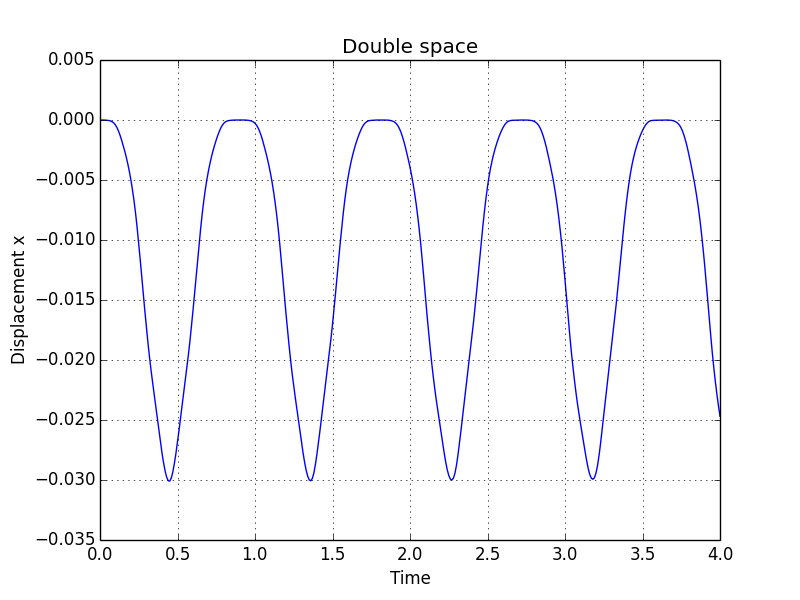
\includegraphics[width=1\linewidth]{med_diff_x.png} 
    \caption{diff x with diffusion term} 
    \vspace{4ex}
  \end{minipage}%%
  \begin{minipage}[b]{0.6\linewidth}
    \centering
    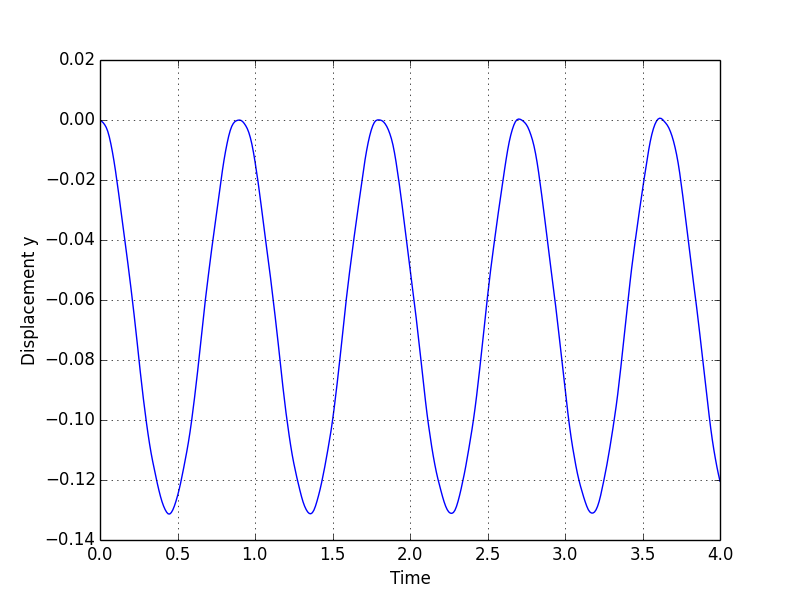
\includegraphics[width=1\linewidth]{med_diff_y.png} 
    \caption{diff y with diffusion term} 
    \vspace{4ex}
  \end{minipage} 
  \begin{minipage}[b]{0.6\linewidth}
    \centering
    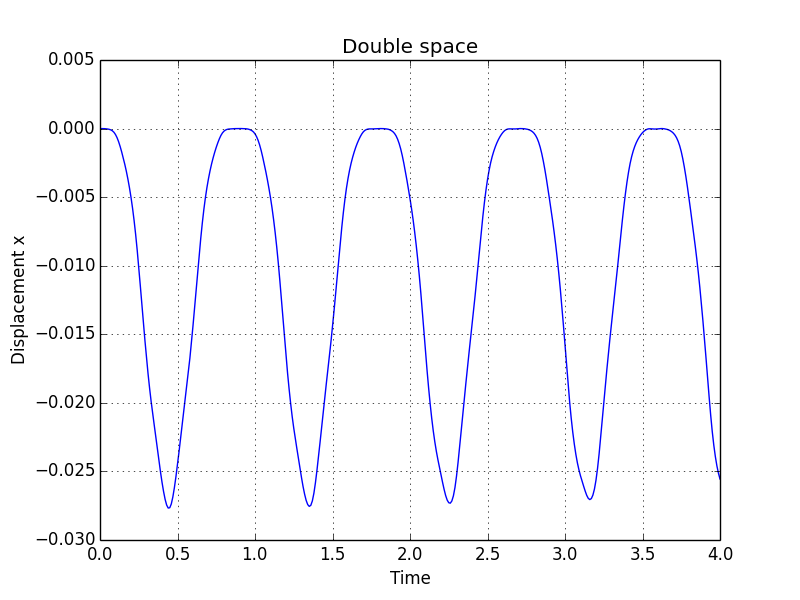
\includegraphics[width=1\linewidth]{uten_diff_x.png} 
    \caption{diff x without diffusion term} 
    \vspace{4ex}
  \end{minipage}%% 
  \begin{minipage}[b]{0.6\linewidth}
    \centering
    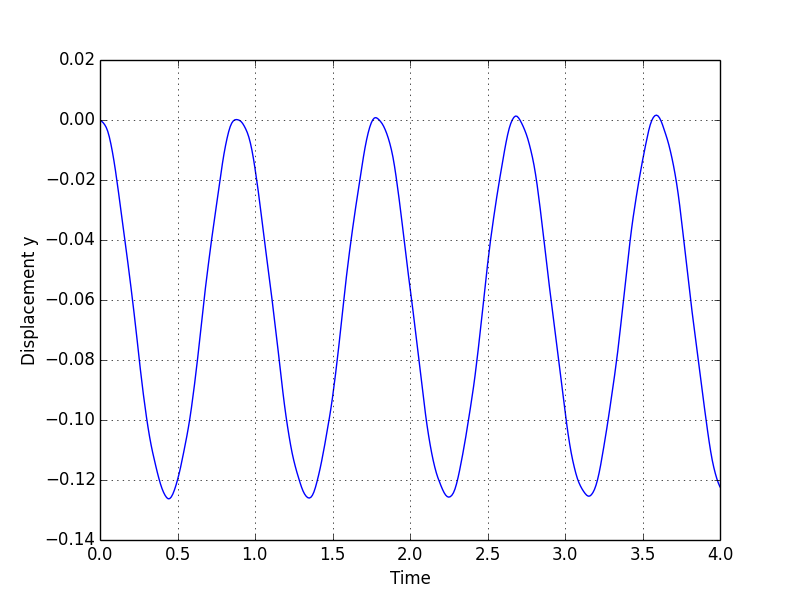
\includegraphics[width=1\linewidth]{uten_diff_y.png} 
    \caption{diff y without diffusion term} 
    \vspace{4ex}
  \end{minipage} 
\end{figure}



\newpage
\newpage 

\subsection*{FSI test}
\begin{table}[ht]
\centering
\caption{Parameters}
\label{my-label}
\begin{tabular}{|l|l|l|l|}
\hline
Parameters & FSI1 & FSI2 & FSI3 \\ \hline
$\rho_f[10^3 \frac{kg}{m^3}]$ & 1 & 1 & 1 \\ \hline
$\nu_f [10^{-3} \frac{m^2}{s}]$ & 1 & 1 & 1 \\ \hline
$u_0$ & 0.2 & 1 & 2 \\ \hline
Re = $\frac{U d}{\nu_f}$ & 20 & 100 & 200 \\ \hline
$\rho_s[10^3 \frac{kg}{m^3}]$ & 1 & 10 & 1 \\ \hline
$\nu_s$ & 0.4 & 0.4 & 0.4 \\ \hline
$\mu_s[10^6 \frac{m^2}{s}]$ & 0.5 & 0.5 & 2 \\ \hline
\end{tabular}
\end{table}
Results: 
\begin{table}[h]
\centering
\caption{FSI 1}
\label{my-label}
\begin{tabular}{|l|l|l|l|l|l|l|}
\hline
Cells & Dofs & ux of A $[x10^{-3}]$ & uy of A $[x10^{-3}]$ & Drag & Lift & Spaces \\ \hline
2698 & 7095 & 0.0234594 & 0.797218  & 14.4963 & 0.915801 & P1-P1-P1 stab= 0.01 \\ \hline
2698 & 23563 & 0.02271 & 0.80288 & 14.1736 & 0.787891 & P2-P2-P1 \\ \hline
10792 & 92992 & 0.0227341 & 0.808792 & 14.1855 & 0.801044 & P2-P2-P1 \\ \hline
43168 & 369448 & 0.227352 & 0.812595 & 14.227 & 0.797242 & P2-P2-P1 \\ \hline
\textbf{ref} & \textbf{ref} & \textbf{0.0227} & \textbf{0.8209} & \textbf{14.295} & \textbf{0.7638} & \textbf{ref} \\ \hline
\end{tabular}
\end{table}



